\bivtask{3D-Clipping für perspektivische Projektion}{12}\label{aufgabe:proj2}
%
Die Projektion aus Aufgabe~\ref{aufgabe:proj1} enthielt noch einige 
Vereinfachungen. So wurde die $z$-Koordinate vernachlässigt und kein 
Clipping in normalisierten Sichtkoordinaten durchgeführt.

Das Rahmenprogramm \texttt{proj2.cc} im Verzeichnis 
\bivfolder{/home/bildgen/Aufgaben/projektion-2} enthält alle Schritte 
für den allgemeinen Fall. Ihre Aufgabe ist, das fehlende Clipping zu 
ergänzen. Sie sollen hierbei keine optimierten Verfahren wie 
Cohen-Sutherland oder Cyrus-Beck-Liang-Barsky auf den 3D-Fall 
übertragen. Gehen Sie einfach von den Parameterdarstellungen der Gerade 
aus, d.\,h.\
\[ x(t) = x₀ + t (x₁ - x₀), \quad y(t) = y₀ + t (y₁ - y₀), \quad
z(t) = z₀ + t (z₁ - z₀), \quad 0 ≤ t ≤ 1 \,\text. \]
Alle notwendigen Parameter und Daten sind im Code vorgegeben. Für jede
Kante wird die Funktion \texttt{clip3D} aufgerufen. Die Endpunkte der 
unbearbeiteten Kante werden als Referenz via \texttt{anf} und 
\texttt{end} übergeben. Führen Sie nun für die jeweilige Kante 
\emph{nacheinander} Clipping an den Clip\-ping\-ebe\-nen in 
normalisierten Sichtkoordinaten aus. Aktualisieren Sie dann 
\texttt{anf} und \texttt{end} mit den neuen Endpunkten der geclippten
Kante.

\begin{enumerate}
\item $-1 ≤ z ≤ z_\text{min}$

      Bestimmen Sie die Schnittpositionen $t₁$, $t₂$ mit der Front- und
      Backplane aus $z(t₁) = -1$ und $z(t₂) = z_\text{min}$. Beachten 
      Sie auch den Sonderfall für Geraden, die in der $x$-$y$-Ebene 
      liegen.

\item\label{it:clip3dzx} $z ≤ x ≤ -z$

      Bestimmen Sie $t₁$, $t₂$ aus $x(t₁) = z(t₁)$ und $x(t₂) = -z(t₂)$.

      Überlegen Sie sich, welche verschiedenen Lagen eine Kante und ihre
      Endpunkte haben kann, so dass sie die zulässige (graue) Fläche
      schneidet (siehe Illustration). Dokumentieren Sie die 
      verschiedenen Fälle entweder in Ihrem Quelltext oder mit Hilfe 
      separater Zeichnungen (oder beides). Beachten Sie hier den 
      Sonderfall, dass die Gerade parallel zur $y$-Achse liegt.

\item $z ≤ y ≤ -z$

      Analog zu Fall~\ref{it:clip3dzx}.
\end{enumerate}

%\clearpage
Testen Sie das Programm mit den Dateien \texttt{Wuerfel?.info} (es ist
jeweils kommentiert, welcher Teil ausgeblendet werden sollte), 
\texttt{Colosseum?.info} und \texttt{sts1.info} sowie den zugehörigen 
Modellen \texttt{Wuerfel.in}, \texttt{Colosseum.in} und \texttt{sts.in}.
Hierzu müssen Sie Ihr Programm z.B. wie folgt aufrufen:
\begin{alltt}
   cat Wuerfel.in Wuerfel1.info | proj2
\end{alltt}

%Beachten Sie, dass die Eingabedateien aus Aufgabe~11 nicht verwendet
%werden können und neue auf der Webseite bereitstehen.
\begin{center}
  \resizebox{250pt}{!}{%
    %% Creator: Inkscape inkscape 0.91, www.inkscape.org
%% PDF/EPS/PS + LaTeX output extension by Johan Engelen, 2010
%% Accompanies image file 'clip3d.pdf' (pdf, eps, ps)
%%
%% To include the image in your LaTeX document, write
%%   \input{<filename>.pdf_tex}
%%  instead of
%%   \includegraphics{<filename>.pdf}
%% To scale the image, write
%%   \def\svgwidth{<desired width>}
%%   \input{<filename>.pdf_tex}
%%  instead of
%%   \includegraphics[width=<desired width>]{<filename>.pdf}
%%
%% Images with a different path to the parent latex file can
%% be accessed with the `import' package (which may need to be
%% installed) using
%%   \usepackage{import}
%% in the preamble, and then including the image with
%%   \import{<path to file>}{<filename>.pdf_tex}
%% Alternatively, one can specify
%%   \graphicspath{{<path to file>/}}
%% 
%% For more information, please see info/svg-inkscape on CTAN:
%%   http://tug.ctan.org/tex-archive/info/svg-inkscape
%%
\begingroup%
  \makeatletter%
  \providecommand\color[2][]{%
    \errmessage{(Inkscape) Color is used for the text in Inkscape, but the package 'color.sty' is not loaded}%
    \renewcommand\color[2][]{}%
  }%
  \providecommand\transparent[1]{%
    \errmessage{(Inkscape) Transparency is used (non-zero) for the text in Inkscape, but the package 'transparent.sty' is not loaded}%
    \renewcommand\transparent[1]{}%
  }%
  \providecommand\rotatebox[2]{#2}%
  \ifx\svgwidth\undefined%
    \setlength{\unitlength}{350.92778675bp}%
    \ifx\svgscale\undefined%
      \relax%
    \else%
      \setlength{\unitlength}{\unitlength * \real{\svgscale}}%
    \fi%
  \else%
    \setlength{\unitlength}{\svgwidth}%
  \fi%
  \global\let\svgwidth\undefined%
  \global\let\svgscale\undefined%
  \makeatother%
  \begin{picture}(1,0.97644639)%
    \put(0,0){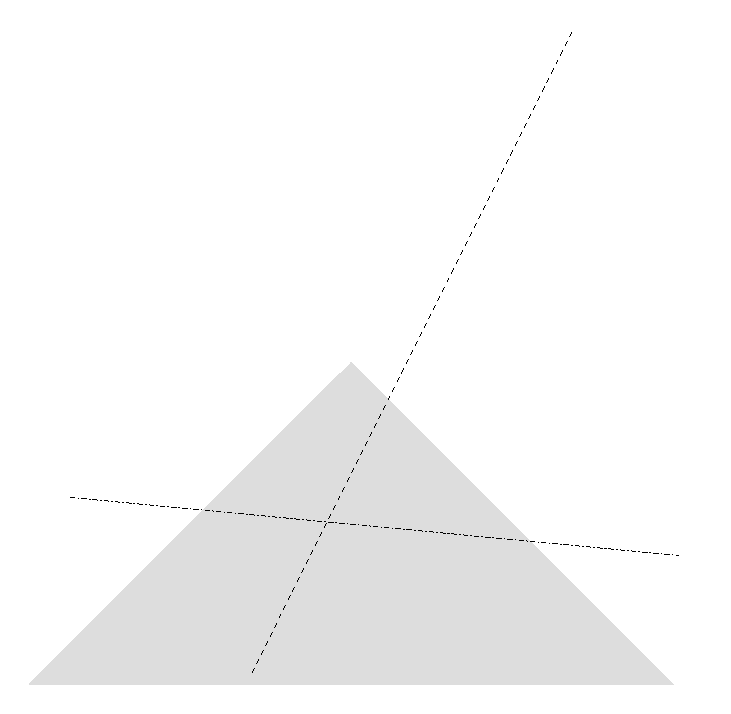
\includegraphics[width=\unitlength,page=1]{clip3d.pdf}}%
    \put(0.56045319,0.42436492){\color[rgb]{0,0,0}\makebox(0,0)[lb]{\smash{$t₂$}}}%
    \put(0.64858009,0.61654935){\color[rgb]{0,0,0}\makebox(0,0)[lb]{\smash{$t₁$}}}%
    \put(0.1762538,0.25624591){\color[rgb]{0,0,0}\makebox(0,0)[lb]{\smash{$t₁$}}}%
    \put(0.7285722,0.24828059){\color[rgb]{0,0,0}\makebox(0,0)[lb]{\smash{$t₂$}}}%
    \put(0,0){\includegraphics[width=\unitlength,page=2]{clip3d.pdf}}%
    \put(0.5045265,0.96092216){\color[rgb]{0,0,0}\makebox(0,0)[lb]{\smash{$z$}}}%
    \put(0.96888748,0.49656119){\color[rgb]{0,0,0}\makebox(0,0)[lb]{\smash{$x$}}}%
    \put(0.89686068,0.07219627){\color[rgb]{0,0,0}\makebox(0,0)[lb]{\smash{$z = -x$}}}%
    \put(0.88872589,0.87279526){\color[rgb]{0,0,0}\makebox(0,0)[lb]{\smash{$z = x$}}}%
  \end{picture}%
\endgroup%
%₁₂
  }%
\end{center}
